\documentclass[10pt,a4paper]{article}
\usepackage{fullpage}
\usepackage[british]{babel}
\usepackage[utf8]{inputenc}
\usepackage[T1]{fontenc}
\usepackage{titling}
\usepackage{graphicx}

% information about author and title
\title{Coursework 1 --- Twitter Analysis}
\author{Alexandre Medeiros}
%\date{\today}

% references become hyperlinks and adds metainfo to the pdf file
\usepackage{hyperref}
\hypersetup{bookmarks=true,
  pdftitle={\thetitle},
  pdfauthor={\theauthor},
  hidelinks
}

\DeclareGraphicsExtensions{.pdf}

\begin{document}
\maketitle

\section{Introduction}

% General introduction
\paragraph*{}
The assignment consist of an analysis of tweets captured during the 2012
Olympics period. Hadoop Map-Reduce was used for the analysis.  The dataset used
in the coursework is available through the ITL's HDFS, on the {\tt
/data/olympictweets} file.

For all the Hadoop jobs, a custom Writable class was used as input, together
with a custom FileInputFormat class, so the map functions could be simplified
and the input parsing, which was common for every problem, could be done
consistently in a separate file.

All the graphs presented in this report were generated with Python scripts using
the pyplot library, the scripts are available in the {\tt scripts} directory of
the submission zip file.

The details for the solution to each problem is given in the next sections.

\section{Text Analysis}

% Short description
\paragraph*{}
The main objective is to analyse the length, in characters, of the tweets. For
this, the histogram on Figure~\ref{fig::text} was generated, with the lengths
aggregated in groups of 5. A job to compute the average length was also created.

\begin{figure}[!b]
    \centering
    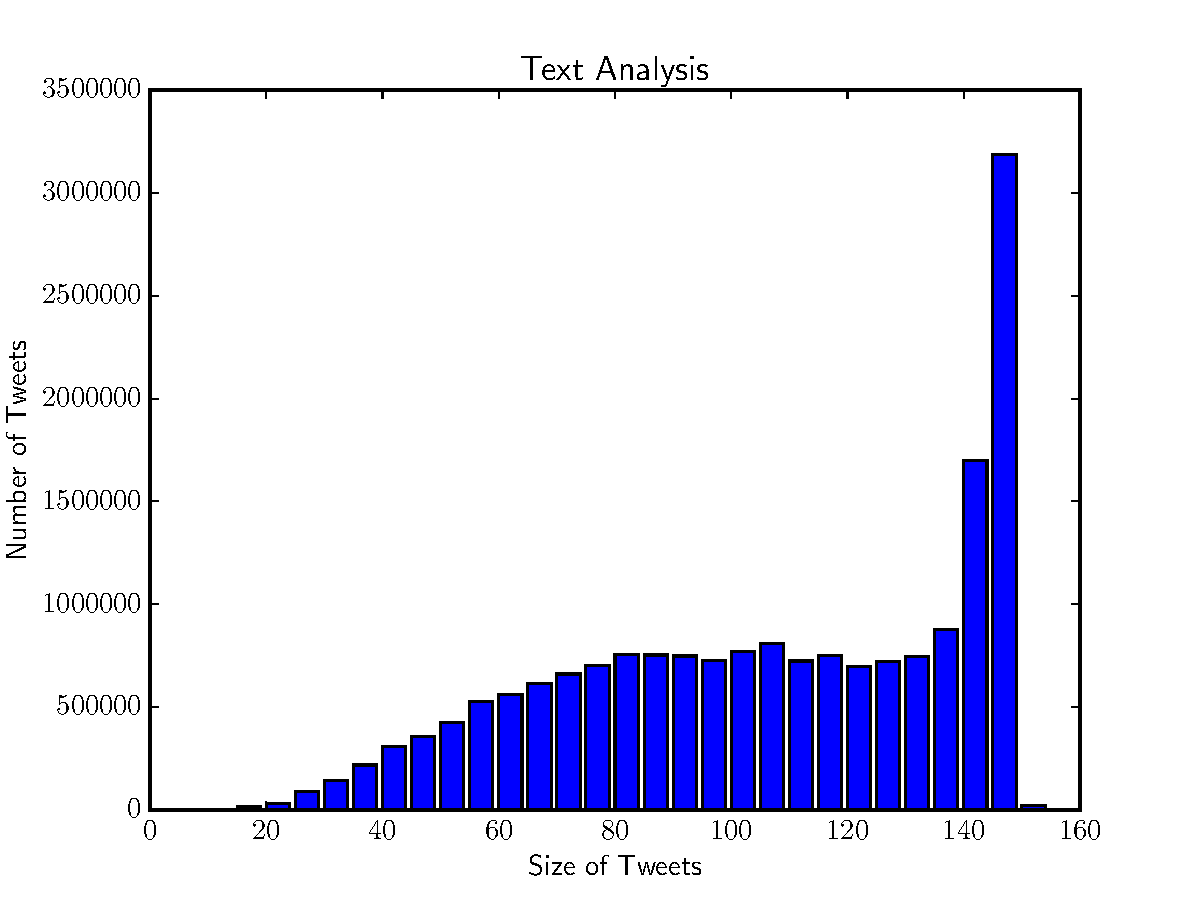
\includegraphics[width=.7\textwidth]{imgs/text-analysis}
    \caption{Tweet length histogram}\label{fig::text}
\end{figure}

% Solution description

\paragraph*{}
For the histogram, all that was needed from the mapper was to classify in which
bin of the histogram a tweet belongs and then emit a pair $(bin, 1)$. The
reducer is a simple count reducer, that sums all the numbers on the values list.

As the reducer is simple and the mapper will emit one pair for each tweet, a
combiner is advisable. And specifically for this count reducer, the combiner may
be the exact same class as the reducer, simplifying the implementation.

\paragraph*{}
To compute the average length, the job was a little different. The mapper
function was responsible for sending a pair $(length, 1)$ as the value for each
tweet with a NullWritable key.

Then the combiner would sum all the lengths and the $1$s, representing the total
length of the tweets and the count.  A single reducer function would sum all the
lengths and counts and then compute the average as $length \div count$.

As tweets only have an integer number of character, the resulting average was
presented as the integer divition. The value found for the average length was
100.

\paragraph*{}
Since there are some tweets that were written in foreign languages, which
contain characters with non-standard encoding, there were some unexpected
values, so we discarded any value above 155 for the histogram, as the count for
these tweets were low. The average was computed normally.

% Describe / analyse the results

\section{Time Analysis}

% Short description
\paragraph*{}
The time analysis of the tweets was made considering the number of tweets per
each day. The graph on Figure~\ref{fig::time} is the result of this analysis.

\begin{figure}[!b]
    \centering
    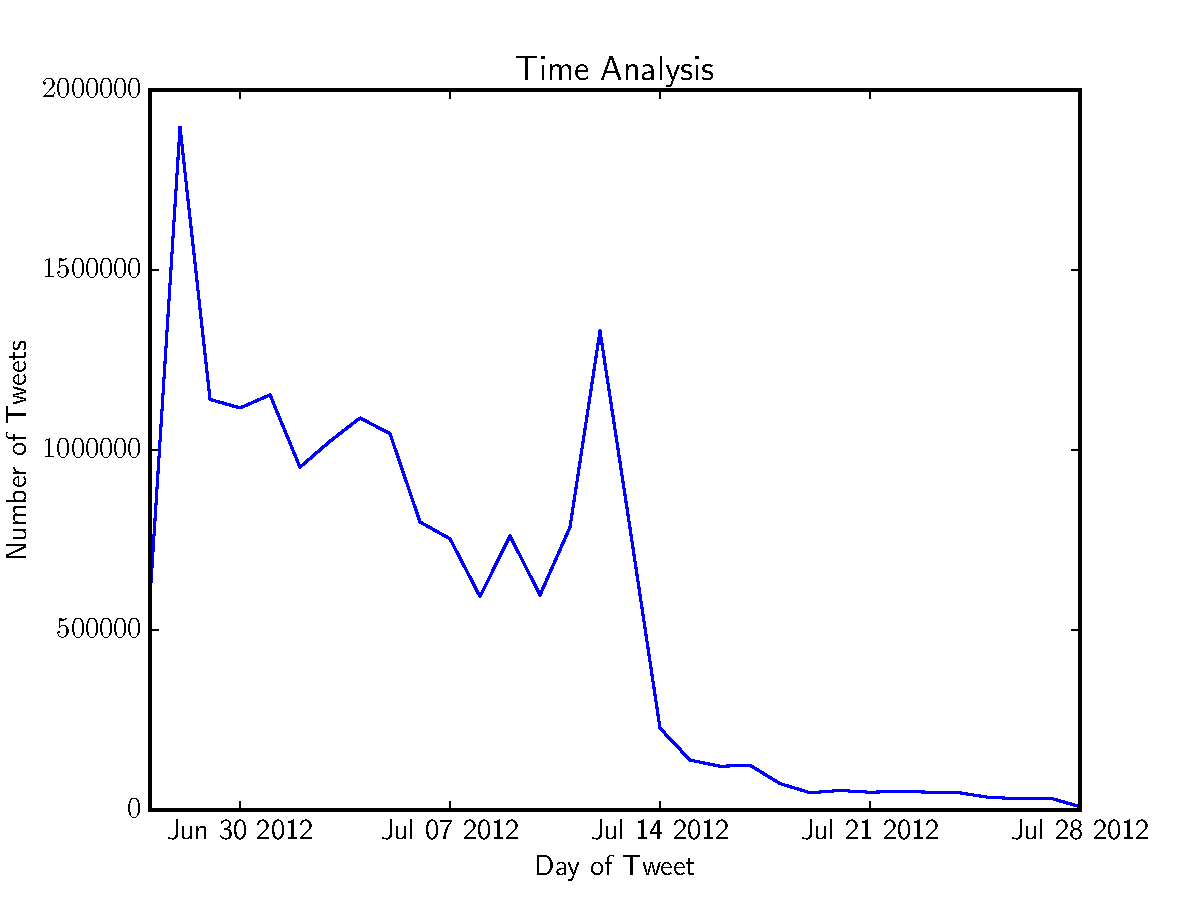
\includegraphics[width=.7\textwidth]{imgs/time-analysis}
    \caption{Olympic Tweets per day}\label{fig::time}
\end{figure}

% Solution description
\paragraph*{}
On the time analysis job, it was needed to get only the day, month and year from
the date. The date internal representation used was a LongWritable, so the first
step was to convert it to a Calendar type, before the needed values could be
read.  The mapper function for this job only needed to compute this conversion
then emit the pair $(day, 1)$.

The reducer was again a simple count reducer. Just like on the length histogram
problem, the same class was used as the reducer and the combiner.

% Describe / analyse the results

\section{Hashtag Analysis}

% Short description
\paragraph*{}
The hashtag analysis consist of finding how many support tweets each team
received, for this, the hashtags used for the tweets were analysed. Hashtags
like {\tt \#goX} and {\tt \#teamX} were considered to represent support tweets
towards the team {\tt X}, e.g., {\tt \#gobrazil} would be a hashtag on a
Brazilian support tweet.

\begin{figure}[!b]
    \centering
    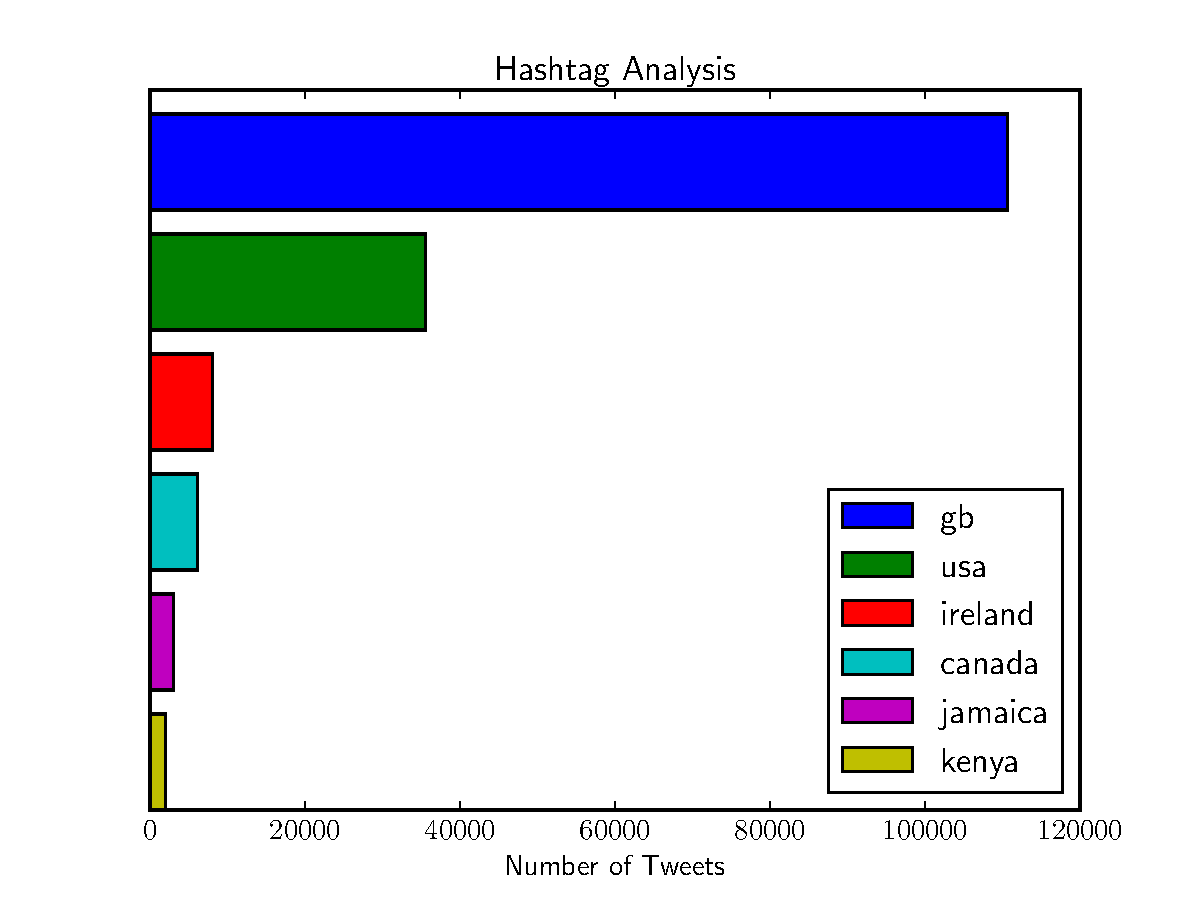
\includegraphics[width=.7\textwidth]{imgs/hashtag-analysis}
    \caption{Top supported countries}\label{fig::hashtag}
\end{figure}

% Solution description
\paragraph*{}
Also for this job, the reduce class was a simple count reducer, which, again,
was also used as a combiner.

The interesting part of this job was how to determine whether a tweet was a
support tweet or not and whose team was it supporting. For this task, Java
regular expressions were used, first a set of patterns were created to represent
a support hashtag, then each hashtag of the tweet is matched against the pattern
considering a priority.

The patterns used, in order of priority were:
\begin{enumerate}
    \item \verb|"^(go)+team(?<t>.*)"|
    \item \verb|"^(go)+(?<t>.*)"|
    \item \verb|"^team(?<t>.*)"|
\end{enumerate}

To sum the support tweet with either one of these patterns, the key the map
function uses as its output is just the group {\tt t} from the Regular
expression, which is the name of the team instead of the whole hashtag.

% Describe / analyse the results

\paragraph*{}
Considering the team in each support tweet, the resulting top teams are
described on the graph on Figure~\ref{fig::hashtag}.

The data used for this graph was manually filtered, because of the patterns
used, some unwanted hashtags were counted, e.g., the hashtags {\tt \#going4gold}
and {\tt \#gold} were considered as support tags for `ing4gold' and `ld',
respectively.

The top 24 most supported teams, can be seen on Table~\ref{tab::hashtag}. The
whole data with the job results can be found on the output directory of the
compressed code submission.

\begin{table}[t]
    \centering
    \caption{Top 24 most supported teams}\label{tab::hashtag}
    \begin{tabular}{|l|l||l|l||l|l|}
        \hline
        Team & Count & Team & Count & Team & Count \\
        \hline\hline
        gb        & 110661 & russia    & 879 & india     & 308  \\
        usa       & 35546  & malaysia  & 786 & mexico    & 298  \\
        ireland   & 8081   & indonesia & 593 & japan     & 284  \\
        canada    & 6101   & australia & 419 & france    & 267  \\
        jamaica   & 3066   & mongolia  & 371 & china     & 266  \\
        kenya     & 2035   & italy     & 369 & hungary   & 240  \\
        canadago  & 2009   & brazil    & 367 & teamusa   & 230  \\
        nigeria   & 936    & aus       & 319 & singapore & 225  \\
        \hline
    \end{tabular}
\end{table}

\end{document}
